\documentclass[a4paper,12pt]{article}

\usepackage[margin=1.2cm]{geometry}
\usepackage{graphicx}
\usepackage{amsmath,amssymb} % symb for \mathbb (C)

\DeclareMathOperator{\Imag}{Im} % works better than \text{Im}\,
\DeclareMathOperator{\Real}{Re}

\pagestyle{empty}

\begin{document}

\section*{Question 7}

\textbf{\large{(a)}} \ Let
\[
  A=\{z:1\leq |z+1|\leq 2\},\qquad
  B=\{\Imag z<0,\ \Real z>-1\},\qquad
  C=\mathbb{C} - A.
\]
\vspace{0.2cm}

\begin{center}
  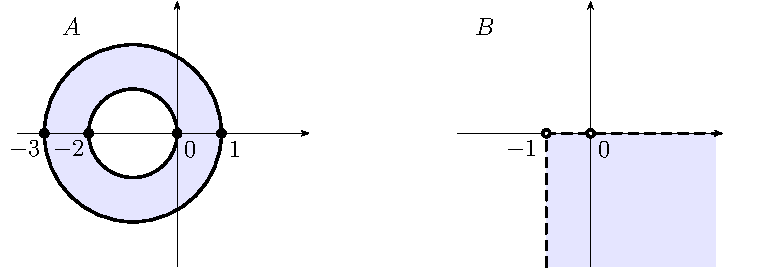
\includegraphics{tikz/Q7a-i-orientation.pdf}
\end{center}

\textbf{\large{(i)}}
\begin{center}
  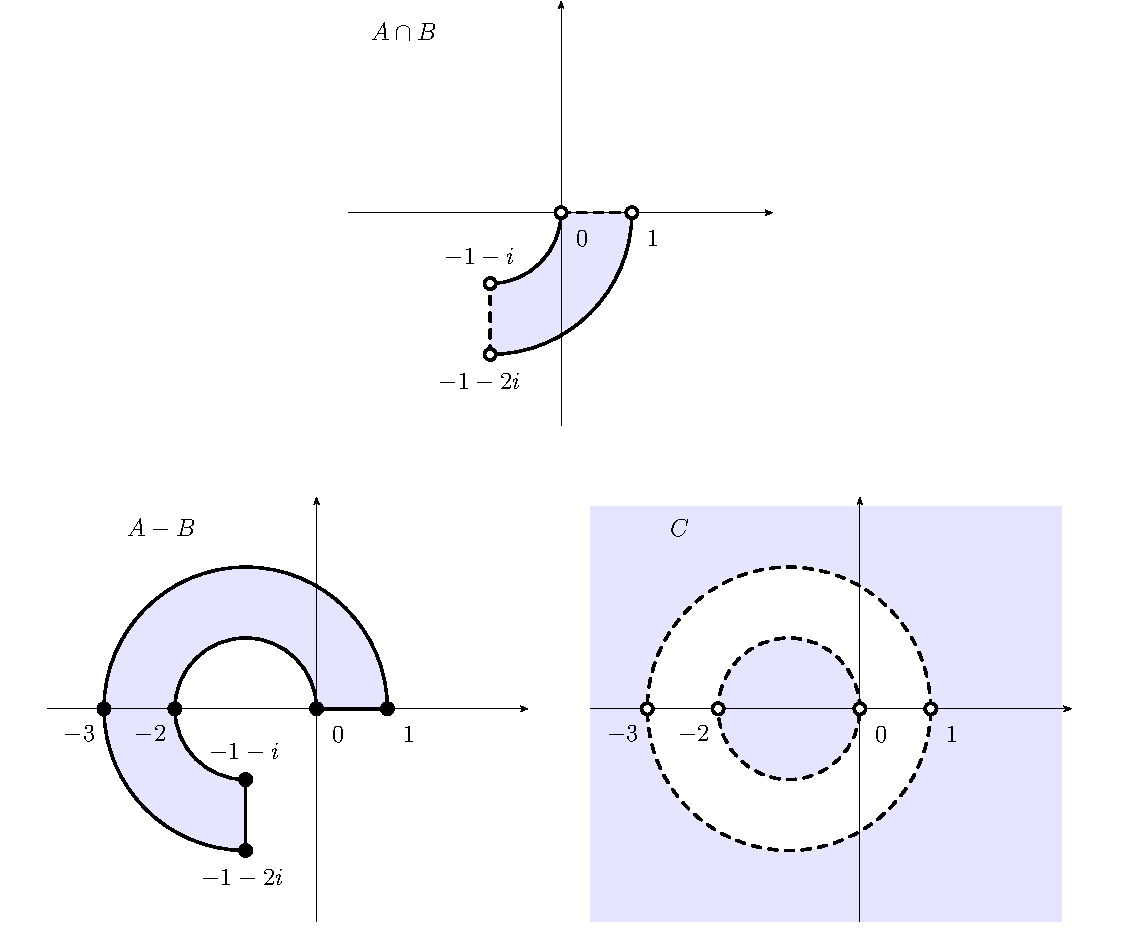
\includegraphics{tikz/Q7a-i-sketches.pdf}
\end{center}

\end{document}
